\chapter{Contexte général} 
\minitoc
\clearpage
\label{sec:organisme}











%\subsection{Contexte et motivations}

%Dans un monde où la connaissance progresse à un rythme exponentiel, tous les domaines technologiques
%(d'informatique, de mathématiques, de physique, de biologie ou de recherche académique...) dépendent %fondamentalement d'un système d'exploitation. Qu'un chercheur développe une application, programme un %mécanisme expérimental, implémente un algorithme ou rédige une publication scientifique, le choix de %son système d'exploitation (OS) influencera profondément son travail et son potentiel de découverte.


\section{Introduction}
La création d'un système d'exploitation personnalisé  est une tâche complexe qui exige une maitrise approfondie des éléments logiciels et matériels. Ce projet vise à concevoir une distribution Linux optimisée spécifiquement adaptée aux chercheurs et aux scientifiques, en incorporant un gestionnaire de paquet dédié, Kraken.

Dans ce premier chapitre, nous allons présenter le cadre général du projet, l'entreprise d'accueil KUSA  ou  sest deroule le stage par la suite le cadre de projet , letude de lexistant presentant la situaton actuelle , la solution propse et finalement la methode du travail adoptee



%presentation kusa -------




\section{Présentation de l'entreprise KUSA}
\label{sec:kusa}

Fondée en 2020 à Sfax (Tunisie), KUSA est une société de services numériques spécialisée dans le développement de solutions technologiques innovantes. Avec une équipe d'experts en ingénierie logicielle et infrastructure IT, l'entreprise accompagne ses clients dans leur transformation numérique à travers une offre complète de services.

\begin{figure}[hbt!]
  \centering
  
\includegraphics[width=10cm,height=5cm]{images_pfe/kusa.png}
  \caption{Logo officiel de la société KUSA}
  \label{fig:kusa_logo}
\end{figure}
\FloatBarrier
\clearpage
\subsection{Profil de l'entreprise}
\begin{itemize}
    \item \textbf{Siège social} : Sfax, Tunisie
    \item \textbf{Année de création} : 2020
    \item \textbf{Secteurs d'intervention} : 
    \begin{itemize}
        \item Industrie 4.0 et IoT
        \item Commerce électronique
        \item Médias numériques
        \item Solutions d'entreprise
    \end{itemize}
    \item \textbf{Effectif} : Équipe pluridisciplinaire de 15+ experts
\end{itemize}

\subsection{Domaines d'expertise et Méthodologie }
KUSA se positionne comme un intégrateur technologique full-stack offrant :

\subsubsection*{ Développement Sur Mesure}
\begin{itemize}
    \item Applications Web (portails, intranet/extranet, e-commerce)
    \item Solutions mobiles cross-platform (iOS, Android)
    \item Intégrations IoT (systèmes à capteurs, appareils connectés)
    \item Développement d'API et systèmes back-end
    \item Architecture microservices
\end{itemize}

%\subsubsection*{B : Maintenance Applicative (TMA)}
%\begin{itemize}
 %   \item \textbf{Maintenance corrective} : 
  %  \begin{itemize}
   %     \item Correction de bugs et anomalies
    %    \item Résolution d'incidents critiques
   % \end{itemize}
    
   % \item \textbf{Maintenance adaptive} :
    %\begin{itemize}
     %   \item Adaptation aux nouvelles réglementations
      %  \item Migration vers de nouveaux environnements techniques
    %\end{itemize}
    
   % \item \textbf{Maintenance perfective} :
   % \begin{itemize}
    %    \item Optimisation des performances système
     %   \item Amélioration de l'expérience utilisateur (UX)
       
    %\end{itemize}
%\end{itemize}

%\subsubsection*{C : Recette Applicative (TRA)}
%\begin{itemize}
 %   \item Tests fonctionnels
  %  \item Tests de performance
   % \item Tests de non-régression
   % \item Scénarios de test automatisés/manuels
%\end{itemize}



%\subsubsection*{D : Ingénierie Système et Réseau}
%\begin{itemize}
 %   \item Configuration de serveurs/réseaux
  %  \item Infrastructure cloud et virtualisation
   % \item Analyse de performances
    %\item Solutions de sécurité/sauvegarde
%\end{itemize}

\subsubsection*{Méthodologie B.O.T}
Kusa utilise un Modèle de gestion de projet en trois phases :
\begin{itemize}
    \item \textbf{Build} : Conception et développement de solutions sur mesure
    \item \textbf{Operate} : Gestion et optimisation opérationnelle
    \item \textbf{Transfer} : Transmission des compétences avec documentation complète
\end{itemize}

%\subsection{Portfolio Clients}
%Principales collaborations récentes :
%\begin{figure}[hbt!]
%  \centering
 % \begin{minipage}[b]{0.18\textwidth}
  %  
\includegraphics[width=\textwidth]{images_pfe/toyota.jpg}
   % \caption{Toyota}
  %\end{minipage}\hfill
  %\begin{minipage}[b]{0.18\textwidth}
  %  
\includegraphics[width=\textwidth]{images_pfe/aqua.png}
  %  \caption{Aquaressort}
  %\end{minipage}\hfill
  %\begin{minipage}[b]{0.18\textwidth}
   % 
\includegraphics[width=\textwidth]{images_pfe/oneticket.png}
   % \caption*{One Ticket}
  %\end{minipage}\hfill
 % \begin{minipage}[b]{0.18\textwidth}
  %  
\includegraphics[width=\textwidth]{images_pfe/diwan.jpg}
   % \caption{Diwan FM}
  %\end{minipage}\hfill
  %\begin{minipage}[b]{0.18\textwidth}
  %  
\includegraphics[width=\textwidth]{images_pfe/tinusdiscount.png}
   % \caption{TuniDiscount}
  %\end{minipage}\hfill
  %\begin{minipage}[b]{0.18\textwidth}
   % 
\includegraphics[width=\textwidth]{images_pfe/fastosh.png}
    %\caption{Fastosh}
  %\end{minipage}
  %\caption{Clients principaux de KUSA}
  %\label{fig:clients}
%\end{figure}
%\FloatBarrier

\section{Contexte du Stage}
\label{sec:contexte_stage}
Ce stage de fin d'études en licence d'informatique (spécialité génie logiciel) s'est déroulé sur quatre mois au sein de KUSA. L'objectif principal consistait à développer une distribution Linux dédiée à la recherche académique et scientifique

Ce projet s'inscrit dans la stratégie d'innovation de KUSA visant à fournir des solutions open source à la communauté scientifique .
\clearpage
%presentation projet ------------------------------------------------
\section{Présentation du projet}

La plupart des développeurs diront que Linux est un système d’exploitation open source. Ceux qui ont des connaissances plus techniques le qualifieront plutôt de noyau.

Pour moi, cependant, Linux n’est pas seulement un système d’exploitation ou un noyau : c’est la liberté, la liberté de créer un système pour un besoin spécifique


\subsection{Problématique et état de l'existant}

\subsubsection{Le paysage actuel des systèmes d'exploitation}
Trois grands types d'OS dominent aujourd'hui :
\begin{itemize}[leftmargin=*,nosep]
\item Windows (développé par Microsoft)
\item macOS (propriété d'Apple)
\item Distributions Linux (basées sur le noyau open source)
\end{itemize}

Les deux premiers, bien que largement utilisés, souffrent de limitations critiques :
\begin{itemize}[leftmargin=*,nosep]
\item \textbf{Fermeture technologique} : Leur code source propriétaire interdit toute modification profonde
\item \textbf{Dépendance aux géants technologiques} : Leur évolution répond à des logiques commerciales plutôt qu'aux besoins spécifiques de la recherche
\end{itemize}

Seul Linux, par sa philosophie  \textbf{open source} et  \textbf{modularité}, offre une liberté totale de personnalisation.

\begin{figure}[htbp]
    \centering
    
\includegraphics[width=0.85\textwidth]{images_pfe/gnulinux.jpeg}
    \caption{GNU LINUX }
    \label{fig:gnulinux}
\end{figure}


\clearpage







Pourtant, les distributions linux existantes imposent un choix cornélien à nous, membres de la communauté académique et scientifique : opter pour une version grand public ou une version spécialisée.
\begin{itemize}[leftmargin=*,nosep]
    \item \textbf{Distributions destinées au grand public} 

   Habituellement, ces distributions sont conçues pour des tâches quotidiennes élémentaires telles que la navigation web ou la gestion d’activités basiques. C’est le cas, par exemple, de Debian ou Fedora, idéales pour les utilisateurs non experts.
Pour les \textbf{transformer}  en stations de travail adaptées à un domaine spécialisé, une configuration complexe et chronophage s’impose — sans aucune garantie de fonctionnement optimal. Nous devons littéralement les \textbf{forcer} à fonctionner comme nous le voulons, ce qui reste très difficile, surtout sans une expertise approfondie en architecture des systèmes d’exploitation.

   .\begin{figure}[hbt!]
  \centering
  \begin{minipage}[b]{0.18\textwidth}
    
\includegraphics[width=\textwidth]{images_pfe/debian.jpg}
    \caption{Debian}
  \end{minipage}\hfill
  \begin{minipage}[b]{0.18\textwidth}
    
\includegraphics[width=\textwidth]{images_pfe/ubuntu.png}
    \caption{Ubuntu}
  \end{minipage}\hfill
  \begin{minipage}[b]{0.18\textwidth}
    
\includegraphics[width=\textwidth]{images_pfe/fedora.jpg}
    \caption{Fedora}
  \end{minipage}\hfill
  \begin{minipage}[b]{0.18\textwidth}
    
\includegraphics[width=\textwidth]{images_pfe/redhat.png}
    \caption{Redhat}
  \end{minipage}\hfill
  \begin{minipage}[b]{0.18\textwidth}
    
\includegraphics[width=\textwidth]{images_pfe/archlinux.png}
    \caption{ArchLinux}
  \end{minipage}\hfill
  
  
  \caption{Distributions destinées au grand public}
  \label{fig:distributions destine au grand public}
\end{figure}
\FloatBarrier

    
   

    \item \textbf{Distributions spécialisées}
    
   Ces distributions ciblent une petite catégorie d’utilisateurs, C’est le cas, par exemple de  Kali Linux , Tails OS ou Blackarch. Généralement, elles sont construites \textbf{ à partir} d’une distribution existante destinée au grand public. L’idée sous-jacente est d’extraire de leur distribution mère certains environnements et outils pour un domaine spécifique, \textbf{sans apporter de modifications radicales}. \\ Par conséquent, elles héritent fondamentalement de la majorité des problèmes inhérents aux distributions grand public. 



   .\begin{figure}[!hbt!]
  \centering
  \begin{minipage}[b]{0.18\textwidth}
    
\includegraphics[width=\textwidth]{images_pfe/kalilinux.png}
    \caption{KaliLinux}
  \end{minipage}\hfill
  \begin{minipage}[b]{0.18\textwidth}
    
\includegraphics[width=\textwidth]{images_pfe/alpine.jpg}
    \caption{Alpine linux }
  \end{minipage}\hfill
  \begin{minipage}[b]{0.18\textwidth}
    
\includegraphics[width=\textwidth]{images_pfe/void.png}
    \caption{Void Linux}
  \end{minipage}\hfill
  \begin{minipage}[b]{0.18\textwidth}
    
\includegraphics[width=\textwidth]{images_pfe/tailsosos.png}
    \caption{Tails os}
  \end{minipage}
  
  \caption{Distributions spécialisées}
  \label{fig:distributions spécialisées}
\end{figure}
\FloatBarrier

   

  \subsection{Quel type de distribution dois-je choisir ?} 
  
\textbf{En tant qu'utilisateur académique et scientifique, quel type de distribution dois-je choisir ?}

Cela peut  surprendre, mais la réponse est : aucun des deux.

\begin{itemize}
    \item \textbf{S’il décide de choisir une distribution dédiée au grand public} (ex. : Debian ou une autre généraliste), il rencontrera inévitablement ces problèmes :
    \begin{enumerate}[label=\Alph*)]
        \item Surcharge logicielle inutile pour son travail.
        \item Configuration complexe pour les outils scientifiques $\rightarrow$ Il ne trouve pas tous les outils de domaine préconstruits et installés. Il devra les ajouter manuellement aux dépôts ou les compiler depuis les sources.
        \item Consommation élevée de ressources $\rightarrow$ Conçue pour le grand public, elle installera par défaut une combinaison d’outils pour tous types d’utilisateurs.
        \item Obligation d’utiliser une interface utilisateur ne correspondant pas à son identité scientifique.
        \item Perte de temps à attendre les mises à jour et nouvelles versions des paquets $\rightarrow$ Les scientifiques ne sont pas la catégorie prioritaire pour les mainteneurs de cette distribution.\\
    \end{enumerate}
    
    \item \textbf{S’il opte pour une distribution spécialisée} (ex. : Kali Linux, tailsos, blackarch) :
    \begin{enumerate}[label=\Alph*)]
        \item Malheureusement, il n’existe pas de distribution spécialisée pour chaque domaine scientifique spécifique.
        \item Impossibilité de s’adapter aux projets multidisciplinaires $\rightarrow$ Exemple : S’il utilise Kali Linux et souhaite exploiter des outils de mathématiques ou de physique, il rencontrera d’énormes difficultés en tant que non-expert en systèmes d’exploitation.
        \item Ces distributions sont conçues pour des niches d’utilisateurs, souvent trop restreintes, ce qui entraîne un manque de mainteneurs motivés $\rightarrow$ Paquets et outils obsolètes ou abandonnés.
    \end{enumerate}
\end{itemize}



\subsection{Analyse des distributions Linux académiques scientifiques}

Il existe déjà plusieurs distributions Linux pour les chercheurs et les scientifiques. La plupart sont \textbf{abandonnées} car elles présentent quelques limitations. Voici ce tableau qui indique les principales distributions scientifiques/académiques existantes et leurs limitations :

\begin{table}[H]
\centering
\begin{tabularx}{\textwidth}{|l|X|l|X|}
\hline
\textbf{Distribution} & \textbf{Public cible} & \textbf{Statut} & \textbf{Problèmes courants} \\
\hline
Scientific Linux & Physique des hautes énergies, analyse de données & Abandonné (2021) & Paquets obsolètes, support matériel limité \\
\hline
Bio-Linux & Génomique, phylogénétique & Abandonné (2016) & Dépendances conflictuelles, dépôts vieillissants \\
\hline
Fedora Scientific & Calcul scientifique général & Actif & Cycle de mise à jour trop rapide, outils limités \\
\hline
Ubuntu Studio & Production multimédia & Actif & Problèmes de compatibilité avec les applications hors multimédia \\
\hline
\end{tabularx}
\caption{Comparaison avec les distributions Linux académiques/scientifiques existantes}
\label{tab:comparaison}
\end{table}




\textbf{Enfin, nous avons cru avoir trouvé une distribution scientifique toujours active et non abandonnée !} \\
Malheureusement, ce n’est pas le cas. Prenons l’exemple de Fedora Scientific, l’une des grandes distributions scientifiques actives :

\begin{itemize}
    \item[A.] Cette distribution est parrainée par une entreprise nommée Red Hat.  une entreprise  qui a récemment choqué la communauté open source en restreignant brusquement l’accès au code source de RHEL (Red Hat Enterprise Linux), ce qui a entraîné une \textbf{perte de confiance}  des utilisateurs. En effet, certains craignent que Fedora Scientific, étant liée à Red Hat, ne soit un jour transformée en produit commercial payant, exigeant un abonnement pour accéder à ses outils
    
    \item[B.] \textbf{Terrain d’essai:} Fedora science est la distribution en amont de RHEL, servant de plateforme de test et d’innovation pour Red Ha.Concrètement, les utilisateurs de Fedora sont des \textbf{rats de laboratoire}  , les nouvelles fonctionnalités, les mises à jour logicielles et les noyaux expérimentaux y sont déployés en premier. Une fois stabilisés et débogués grâce aux retours de la communauté, ces paquets sont intégrés à RHEL
    
    \item[B.] \textbf{ Outils préinstallés problématiques :} Elle inclut une suite étendue d’outils scientifiques préinstallés, entraînant :
        \begin{itemize}
            \item Un gaspillage d’espace disque .
            \item Conflits de dépendances et ralentissements sur machines 
        \end{itemize}
    
  \item[C.] \textbf{Cycle de publication :} Fedora Science publie de nouvelles versions tous les 6 mois : donc il devra attendre six mois pour toute mise à jour du système, noyau et pilotes inclus.

    \item[D.] \textbf{Limitations du gestionnaire de paquets :}  DNF est plus lent et limité en raison de ses dépôts , ce qui ralentit la résolution des dépendances.
    
  \item[E.]  \textbf{Environnements non isolés et dépendances externes :} Dépendance à des logiciels tiers et services externes (non maintenus par l’équipe Fedora). De plus, aucune séparation n’existe entre les environnements de chaque domaine. Il héritera donc de dizaines d’outils inutiles pour un besoin spécifique.
\end{itemize}


\textbf{Les problèmes principaux sont :}
\begin{enumerate}[label=\alph*)]
    \item Complexité de configuration
    \item Problèmes de pilotes et compatibilité
    \item Spécialisation mono-domaine
    \item Limitations de personnalisation de l’interface
    \item Courbe d’apprentissage difficile
    \item Problèmes de dépendances
    \item Risque d’abandon à tout moment
    \item Problèmes de confiance au sein de la communauté open source
\end{enumerate}
\clearpage
\subsection{Solution proposée par notre distribution}

\subsubsection{Le paradoxe à résoudre}
\textbf{Comment concilier deux exigences apparemment contradictoires ?}
\begin{itemize}
\item \textbf{Préserver les fondamentaux }: Assurer toutes les fonctions de base d'un OS moderne
\item \textbf{Offrir une flexibilité radicale }: Permettre à l'OS de se transformer en :
\begin{itemize}
\item Laboratoire de mathématiques
\item Station de développement (mobile, web, desktop, cybersécurité)
\item Environnement de simulation physique
\item Plateforme d'analyse génomique
\item Environnement de physique computationnelle
\item Station de développement IA/ML
\end{itemize}
\end{itemize}
\textbf{Cohabitation sans conflits :} Tous ces environnements spécialisés peuvent fonctionner simultanément sur le même système, sans interférences ni incompatibilités \\ 
\\
\\

 Pour répondre à ces défis, nous développons une distribution Linux adaptée aux besoins des scientifiques et chercheurs, visant à combler les lacunes problématiques des distributions scientifiques existantes


\subsection{Pourquoi choisir Kraken OS ?}

\textbf{Kraken OS} a priorisé la résolution méthodique des lacunes et problématiques critiques recensées dans les distributions existantes, grâce à des mécanismes novateurs et une refonte philosophique profonde de son architecture

\begin{itemize}
    
    
    \item \textbf{Comment résolvons-nous le problème des dépendances ?}\\ Pour éviter la dépendance aux distributions mères dédiées au grand public, nous construisons notre système depuis les sources, assurant un \textbf{contrôle total}. \\
    
    \item \textbf{Comment résolvons-nous le problème de stabilité ?}\\ Nous avons implémenté un nouveau gestionnaire de paquets utilisant un mécanisme hybride, offrant à la fois des mises à jour en rolling release et une base stable. \\
    
    \item \textbf{Comment résolvons-nous le problème des paquets inutiles préinstallés ?}\\ Un mécanisme de sélection modulaire permet de choisir strictement les paquets par domaine scientifique, garantissant une séparation claire.\\
    
    \item \textbf{Comment résolvons-nous le problème des multi-environnements ?}\\ Un système de basculement fluide entre environnements spécialisés (mathématiques, informatique, physique, etc.) a été intégré.
    \\
    \item \textbf{Comment résolvons-nous le problème des limitations de personnalisation ?}\\ Nous fournissons des environnements graphiques complets adaptés à l’identité de chaque domaine. \\
    \textbf{Note :} L’utilisateur dispose également de tous les outils pour personnaliser son environnement selon ses besoins.
    \\
    \item \textbf{Comment résolvons-nous le problème de confiance ?} \\L’intégralité du projet est développée sous une philosophie open source stricte.\\
    
    \item \textbf{Comment résolvons-nous le problème de complexité de configuration ?}\\ Un mécanisme de post-installation automatisé dans le gestionnaire de paquets gère toutes les configurations nécessaires (fichiers de paquets, liens symboliques, entrées de bureau, activation au démarrage, etc.).\\
    \item \textbf{Comment résolvons-nous le problème de d’apprentissage difficile ?}\\Des tutoriels interactifs complets, organisés par domaine scientifique et par outil, sont intégrés au système.\\
\end{itemize}
\clearpage
 \subsection{ Pourquoi Kraken OS redéfinit les standards des systèmes scientifiques ?} \\ \\
Cette distribution sera capable de :
\begin{enumerate}[label=\alph*)]
\item Assurer le bon fonctionnement des fondamentaux d’un système d’exploitation moderne :
\begin{itemize}
\item Gestion mémoire 
\item Contrôle des périphériques et pilotes
\item Orchestration des processus et threads
\item Système de fichiers évolutif
\end{itemize}

\item Fournir une interface personnalisable et conviviale  :
\begin{itemize}
\item Gestionnaires de fenêtres personnalisés (GNOME/KDE)
\item Profils visuels par discipline (MATH ,PHYSIQUE , INFORMATIQUE ...)
\end{itemize}

\item Fournir tous les outils préconfigurés nécessaires via le gestionnaire de paquets "Kraken" :
\begin{itemize}
\item Catalogue modulaire validé (paquets validés par la communauté scientifique)
\item Gestion des interdépendances multi-domaines
\end{itemize}

\item Environnement sécurisé :
\begin{itemize}
\item Isolation des expérimentations critiques
\item Authentification, Autorisation, Audit
\end{itemize}

\item Faciliter l’installation et la configuration des outils de recherche : 
\begin{itemize}
\item Assistants d'installation contextuels (workflows guidés par domaine)
\item Configuration automatique des environnements
\end{itemize}

\item Flexibilité interdisciplinaire :
\begin{itemize}
\item Bascules rapides entre domaines scientifiques
\item Gestion des conflits de dépendances multi-domaines
\end{itemize}

\item Optimisation des performances scientifiques :
\begin{itemize}
\item Compilation pour calcul intensif
\item Gestion des ressources GPU/CPU
\end{itemize}

\item Compatibilité matérielle :
\begin{itemize}
\item Pilotes pour instruments de laboratoire
\item Support des protocoles scientifiques
\end{itemize}

\item Documentation :
\begin{itemize}
\item Aide intégrée par discipline
\item Tutoriels interactifs par domaine \\ 
 \\ 
 \\
\end{itemize}
\end{enumerate}


\textbf{
Kraken OS est bien plus qu’un simple système d’exploitation : c’est l’environnement ultime pour un poste de travail scientifique ou académique, quelle que soit la discipline concernée. Les besoins en recherche et les exigences professionnelles sont placés au cœur de la philosophie du système.
}







\section{Méthodologie de travail}
Durant notre stage chez KUSA, nous avons adopté la méthodologie Agile, plus précisément le cadre Scrum pour résoudre notre probléme et trouver des solutions pour faciliter n'importe quelle tâche . 
%\subsection{Présentation de la méthode SCRUM}

Scrum signifie mêlée en français, ce cadre méthodologique agile révolutionne la manière dont on gére un projet dont lequel l'équipe se réuni le plus souvent possible afin de vérifier que le projet avance correctement. Il permet de délivrer et de modifier un projet, un produit ou une foctionnalité très rapidement. 

L'équipe Scrum est composée de:
\begin{itemize}
    \item 	Product Owner :

Il porte la vision de produit à créer, et c'est donc souvent un expert de domaine. l travaille en collaboration directe avec l’équipe de développement et a notamment la charge de remplir le Backlogproduit et de déterminer la priorité des user stories à réaliser.

      \item 	Scrum Master :

c'et un membre de la part entiére de l'équipe projet, et il doit maîtriser Scrum car il est charger de garantir que la méthodologie est appliquée correctement.

        \item Équipe de développement :

Elle regroupe les personnes qui seront responsabe de la de la mise en oeuvre des besoins des clients. Cette équipe est habituellement composée de développeurs, testeurs et d'autres membre pertinents .

\end{itemize}

La figure représente à la fois les différents  rôles de Scrum que nous venons de montrer et le déroulement de processus .

\label{sec:hotspot}
La figure \ref{fig:scrum} représente le cycle de vie SCRUM.
\begin{figure}[hbt!]
  \centering
  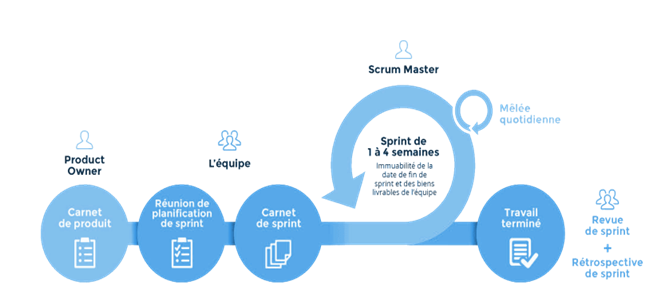
\includegraphics[width=17cm]{images_pfe/scrum.png}
  \caption{Cycle de vie SCRUM.}
  \label{fig:scrum}
\end{figure}
\FloatBarrier

\section{Conclusion}
Ce chapitre présente une étude préliminaire du projet dans lequel  nous avons d'abord exposé le cadre et la problématique et les motivations ayant conduit au développement de cette  distribution Linux.

Dans le prochain chapitre, nous allons examiner la phase d'architecture et les choix techniques qui ont orienté la conception du système et du gestionnaire du paquets Kraken.
 
\medskip



      









  
            

        




  















